\documentclass[1p]{elsarticle_modified}
%\bibliographystyle{elsarticle-num}

%\usepackage[colorlinks]{hyperref}
%\usepackage{abbrmath_seonhwa} %\Abb, \Ascr, \Acal ,\Abf, \Afrak
\usepackage{amsfonts}
\usepackage{amssymb}
\usepackage{amsmath}
\usepackage{amsthm}
\usepackage{scalefnt}
\usepackage{amsbsy}
\usepackage{kotex}
\usepackage{caption}
\usepackage{subfig}
\usepackage{color}
\usepackage{graphicx}
\usepackage{xcolor} %% white, black, red, green, blue, cyan, magenta, yellow
\usepackage{float}
\usepackage{setspace}
\usepackage{hyperref}

\usepackage{tikz}
\usetikzlibrary{arrows}

\usepackage{multirow}
\usepackage{array} % fixed length table
\usepackage{hhline}

%%%%%%%%%%%%%%%%%%%%%
\makeatletter
\renewcommand*\env@matrix[1][\arraystretch]{%
	\edef\arraystretch{#1}%
	\hskip -\arraycolsep
	\let\@ifnextchar\new@ifnextchar
	\array{*\c@MaxMatrixCols c}}
\makeatother %https://tex.stackexchange.com/questions/14071/how-can-i-increase-the-line-spacing-in-a-matrix
%%%%%%%%%%%%%%%

\usepackage[normalem]{ulem}

\newcommand{\msout}[1]{\ifmmode\text{\sout{\ensuremath{#1}}}\else\sout{#1}\fi}
%SOURCE: \msout is \stkout macro in https://tex.stackexchange.com/questions/20609/strikeout-in-math-mode

\newcommand{\cancel}[1]{
	\ifmmode
	{\color{red}\msout{#1}}
	\else
	{\color{red}\sout{#1}}
	\fi
}

\newcommand{\add}[1]{
	{\color{blue}\uwave{#1}}
}

\newcommand{\replace}[2]{
	\ifmmode
	{\color{red}\msout{#1}}{\color{blue}\uwave{#2}}
	\else
	{\color{red}\sout{#1}}{\color{blue}\uwave{#2}}
	\fi
}

\newcommand{\Sol}{\mathcal{S}} %segment
\newcommand{\D}{D} %diagram
\newcommand{\A}{\mathcal{A}} %arc


%%%%%%%%%%%%%%%%%%%%%%%%%%%%%5 test

\def\sl{\operatorname{\textup{SL}}(2,\Cbb)}
\def\psl{\operatorname{\textup{PSL}}(2,\Cbb)}
\def\quan{\mkern 1mu \triangleright \mkern 1mu}

\theoremstyle{definition}
\newtheorem{thm}{Theorem}[section]
\newtheorem{prop}[thm]{Proposition}
\newtheorem{lem}[thm]{Lemma}
\newtheorem{ques}[thm]{Question}
\newtheorem{cor}[thm]{Corollary}
\newtheorem{defn}[thm]{Definition}
\newtheorem{exam}[thm]{Example}
\newtheorem{rmk}[thm]{Remark}
\newtheorem{alg}[thm]{Algorithm}

\newcommand{\I}{\sqrt{-1}}
\begin{document}

%\begin{frontmatter}
%
%\title{Boundary parabolic representations of knots up to 8 crossings}
%
%%% Group authors per affiliation:
%\author{Yunhi Cho} 
%\address{Department of Mathematics, University of Seoul, Seoul, Korea}
%\ead{yhcho@uos.ac.kr}
%
%
%\author{Seonhwa Kim} %\fnref{s_kim}}
%\address{Center for Geometry and Physics, Institute for Basic Science, Pohang, 37673, Korea}
%\ead{ryeona17@ibs.re.kr}
%
%\author{Hyuk Kim}
%\address{Department of Mathematical Sciences, Seoul National University, Seoul 08826, Korea}
%\ead{hyukkim@snu.ac.kr}
%
%\author{Seokbeom Yoon}
%\address{Department of Mathematical Sciences, Seoul National University, Seoul, 08826,  Korea}
%\ead{sbyoon15@snu.ac.kr}
%
%\begin{abstract}
%We find all boundary parabolic representation of knots up to 8 crossings.
%
%\end{abstract}
%\begin{keyword}
%    \MSC[2010] 57M25 
%\end{keyword}
%
%\end{frontmatter}

%\linenumbers
%\tableofcontents
%
\newcommand\colored[1]{\textcolor{white}{\rule[-0.35ex]{0.8em}{1.4ex}}\kern-0.8em\color{red} #1}%
%\newcommand\colored[1]{\textcolor{white}{ #1}\kern-2.17ex	\textcolor{white}{ #1}\kern-1.81ex	\textcolor{white}{ #1}\kern-2.15ex\color{red}#1	}

{\Large $\underline{10_{81}~(K10a_{7})}$}

\setlength{\tabcolsep}{10pt}
\renewcommand{\arraystretch}{1.6}
\vspace{1cm}\begin{tabular}{m{100pt}>{\centering\arraybackslash}m{274pt}}
\multirow{5}{120pt}{
	\centering
	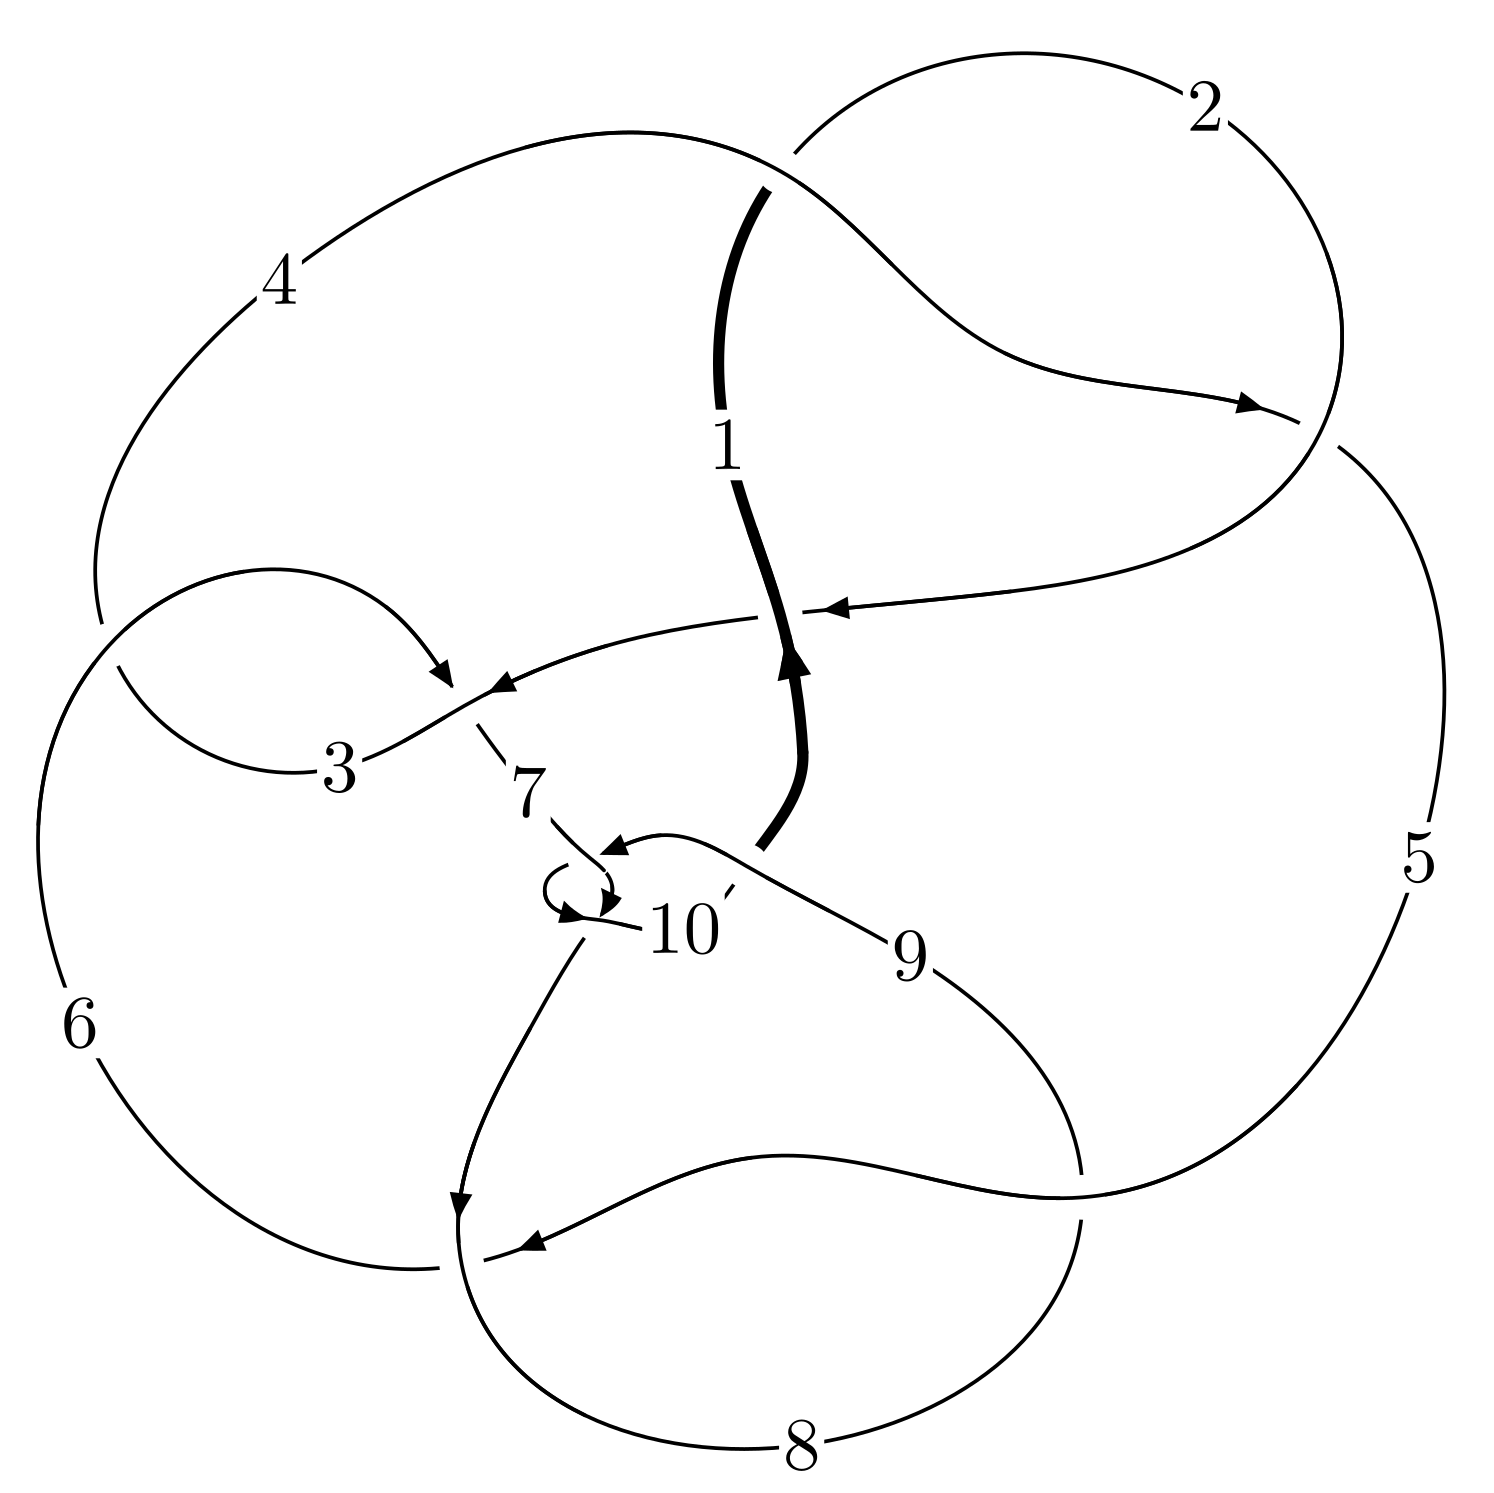
\includegraphics[width=112pt]{../../../GIT/diagram.site/Diagrams/png/165_10_81.png}\\
\ \ \ A knot diagram\footnotemark}&
\allowdisplaybreaks
\textbf{Linearized knot diagam} \\
\cline{2-2}
 &
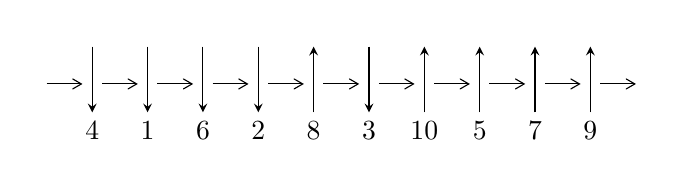
\begin{tikzpicture}[x=20pt, y=17pt]
	% nodes
	\node (C0) at (0, 0) {};
	\node (C1) at (1, 0) {};
	\node (C1U) at (1, +1) {};
	\node (C1D) at (1, -1) {4};

	\node (C2) at (2, 0) {};
	\node (C2U) at (2, +1) {};
	\node (C2D) at (2, -1) {1};

	\node (C3) at (3, 0) {};
	\node (C3U) at (3, +1) {};
	\node (C3D) at (3, -1) {6};

	\node (C4) at (4, 0) {};
	\node (C4U) at (4, +1) {};
	\node (C4D) at (4, -1) {2};

	\node (C5) at (5, 0) {};
	\node (C5U) at (5, +1) {};
	\node (C5D) at (5, -1) {8};

	\node (C6) at (6, 0) {};
	\node (C6U) at (6, +1) {};
	\node (C6D) at (6, -1) {3};

	\node (C7) at (7, 0) {};
	\node (C7U) at (7, +1) {};
	\node (C7D) at (7, -1) {10};

	\node (C8) at (8, 0) {};
	\node (C8U) at (8, +1) {};
	\node (C8D) at (8, -1) {5};

	\node (C9) at (9, 0) {};
	\node (C9U) at (9, +1) {};
	\node (C9D) at (9, -1) {7};

	\node (C10) at (10, 0) {};
	\node (C10U) at (10, +1) {};
	\node (C10D) at (10, -1) {9};
	\node (C11) at (11, 0) {};

	% arrows
	\draw[->,>={angle 60}]
	(C0) edge (C1) (C1) edge (C2) (C2) edge (C3) (C3) edge (C4) (C4) edge (C5) (C5) edge (C6) (C6) edge (C7) (C7) edge (C8) (C8) edge (C9) (C9) edge (C10) (C10) edge (C11) ;	\draw[->,>=stealth]
	(C1U) edge (C1D) (C2U) edge (C2D) (C3U) edge (C3D) (C4U) edge (C4D) (C5D) edge (C5U) (C6U) edge (C6D) (C7D) edge (C7U) (C8D) edge (C8U) (C9D) edge (C9U) (C10D) edge (C10U) ;
	\end{tikzpicture} \\
\hhline{~~} \\& 
\textbf{Solving Sequence} \\ \cline{2-2} 
 &
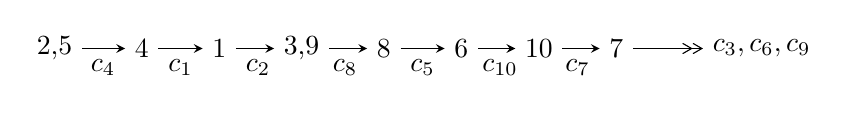
\begin{tikzpicture}[x=28pt, y=7pt]
	% node
	\node (A0) at (-1/8, 0) {2,5};
	\node (A1) at (1, 0) {4};
	\node (A2) at (2, 0) {1};
	\node (A3) at (49/16, 0) {3,9};
	\node (A4) at (33/8, 0) {8};
	\node (A5) at (41/8, 0) {6};
	\node (A6) at (49/8, 0) {10};
	\node (A7) at (57/8, 0) {7};
	\node (C1) at (1/2, -1) {$c_{4}$};
	\node (C2) at (3/2, -1) {$c_{1}$};
	\node (C3) at (5/2, -1) {$c_{2}$};
	\node (C4) at (29/8, -1) {$c_{8}$};
	\node (C5) at (37/8, -1) {$c_{5}$};
	\node (C6) at (45/8, -1) {$c_{10}$};
	\node (C7) at (53/8, -1) {$c_{7}$};
	\node (A8) at (9, 0) {$c_{3},c_{6},c_{9}$};

	% edge
	\draw[->,>=stealth]	
	(A0) edge (A1) (A1) edge (A2) (A2) edge (A3) (A3) edge (A4) (A4) edge (A5) (A5) edge (A6) (A6) edge (A7) ;
	\draw[->>,>={angle 60}]	
	(A7) edge (A8);
\end{tikzpicture} \\ 

\end{tabular} \\

\footnotetext{
The image of knot diagram is generated by the software ``\textbf{Draw programme}" developed by Andrew Bartholomew(\url{http://www.layer8.co.uk/maths/draw/index.htm\#Running-draw}), where we modified some parts for our purpose(\url{https://github.com/CATsTAILs/LinksPainter}).
}\phantom \\ \newline 
\centering \textbf{Ideals for irreducible components\footnotemark of $X_{\text{par}}$} 
 
\begin{align*}
I^u_{1}&=\langle 
-1.38501\times10^{15} u^{47}+7.04930\times10^{15} u^{46}+\cdots+1.31625\times10^{15} b+3.65379\times10^{15},\\
\phantom{I^u_{1}}&\phantom{= \langle  }1.00335\times10^{16} u^{47}-3.95579\times10^{16} u^{46}+\cdots+2.63249\times10^{15} a+1.73053\times10^{16},\;u^{48}-5 u^{47}+\cdots+10 u+1\rangle \\
I^u_{2}&=\langle 
b,\;- u^2+a+2 u-1,\;u^3- u^2+1\rangle \\
I^u_{3}&=\langle 
a^2+b+2 a+1,\;a^3+2 a^2+a+1,\;u+1\rangle \\
\\
\end{align*}
\raggedright * 3 irreducible components of $\dim_{\mathbb{C}}=0$, with total 54 representations.\\
\footnotetext{All coefficients of polynomials are rational numbers. But the coefficients are sometimes approximated in decimal forms when there is not enough margin.}
\newpage
\renewcommand{\arraystretch}{1}
\centering \section*{I. $I^u_{1}= \langle -1.39\times10^{15} u^{47}+7.05\times10^{15} u^{46}+\cdots+1.32\times10^{15} b+3.65\times10^{15},\;1.00\times10^{16} u^{47}-3.96\times10^{16} u^{46}+\cdots+2.63\times10^{15} a+1.73\times10^{16},\;u^{48}-5 u^{47}+\cdots+10 u+1 \rangle$}
\flushleft \textbf{(i) Arc colorings}\\
\begin{tabular}{m{7pt} m{180pt} m{7pt} m{180pt} }
\flushright $a_{2}=$&$\begin{pmatrix}0\\u\end{pmatrix}$ \\
\flushright $a_{5}=$&$\begin{pmatrix}1\\0\end{pmatrix}$ \\
\flushright $a_{4}=$&$\begin{pmatrix}1\\- u^2\end{pmatrix}$ \\
\flushright $a_{1}=$&$\begin{pmatrix}u\\- u^3+u\end{pmatrix}$ \\
\flushright $a_{3}=$&$\begin{pmatrix}- u^3\\u^5- u^3+u\end{pmatrix}$ \\
\flushright $a_{9}=$&$\begin{pmatrix}-3.81140 u^{47}+15.0268 u^{46}+\cdots+36.2869 u-6.57375\\1.05225 u^{47}-5.35561 u^{46}+\cdots-25.7273 u-2.77592\end{pmatrix}$ \\
\flushright $a_{8}=$&$\begin{pmatrix}-4.86364 u^{47}+20.3824 u^{46}+\cdots+62.0142 u-3.79783\\1.05225 u^{47}-5.35561 u^{46}+\cdots-25.7273 u-2.77592\end{pmatrix}$ \\
\flushright $a_{6}=$&$\begin{pmatrix}0.828554 u^{47}-0.00856335 u^{46}+\cdots+28.0123 u-1.38653\\-2.29509 u^{47}+7.50970 u^{46}+\cdots+3.57759 u+0.200750\end{pmatrix}$ \\
\flushright $a_{10}=$&$\begin{pmatrix}2.99681 u^{47}-12.6887 u^{46}+\cdots-38.0813 u+3.39699\\0.302246 u^{47}-0.355609 u^{46}+\cdots+8.52273 u+0.974080\end{pmatrix}$ \\
\flushright $a_{7}=$&$\begin{pmatrix}0.0322954 u^{47}+0.330979 u^{46}+\cdots+8.02219 u-3.03662\\-0.302246 u^{47}+0.355609 u^{46}+\cdots-8.52273 u-0.974080\end{pmatrix}$\\&\end{tabular}
\flushleft \textbf{(ii) Obstruction class $= -1$}\\~\\
\flushleft \textbf{(iii) Cusp Shapes $= \frac{2572719667737379}{1316245742897122} u^{47}-\frac{14240246736967463}{1316245742897122} u^{46}+\cdots-\frac{66418667522566225}{1316245742897122} u+\frac{3102450479488985}{658122871448561}$}\\~\\
\newpage\renewcommand{\arraystretch}{1}
\flushleft \textbf{(iv) u-Polynomials at the component}\newline \\
\begin{tabular}{m{50pt}|m{274pt}}
Crossings & \hspace{64pt}u-Polynomials at each crossing \\
\hline $$\begin{aligned}c_{1},c_{4}\end{aligned}$$&$\begin{aligned}
&u^{48}-5 u^{47}+\cdots+10 u+1
\end{aligned}$\\
\hline $$\begin{aligned}c_{2}\end{aligned}$$&$\begin{aligned}
&u^{48}+23 u^{47}+\cdots+180 u+1
\end{aligned}$\\
\hline $$\begin{aligned}c_{3},c_{6}\end{aligned}$$&$\begin{aligned}
&u^{48}-2 u^{47}+\cdots+28 u-8
\end{aligned}$\\
\hline $$\begin{aligned}c_{5},c_{8}\end{aligned}$$&$\begin{aligned}
&u^{48}+2 u^{47}+\cdots-28 u-8
\end{aligned}$\\
\hline $$\begin{aligned}c_{7},c_{9}\end{aligned}$$&$\begin{aligned}
&u^{48}+5 u^{47}+\cdots-10 u+1
\end{aligned}$\\
\hline $$\begin{aligned}c_{10}\end{aligned}$$&$\begin{aligned}
&u^{48}-23 u^{47}+\cdots-180 u+1
\end{aligned}$\\
\hline
\end{tabular}\\~\\
\newpage\renewcommand{\arraystretch}{1}
\flushleft \textbf{(v) Riley Polynomials at the component}\newline \\
\begin{tabular}{m{50pt}|m{274pt}}
Crossings & \hspace{64pt}Riley Polynomials at each crossing \\
\hline $$\begin{aligned}c_{1},c_{4},c_{7}\\c_{9}\end{aligned}$$&$\begin{aligned}
&y^{48}-23 y^{47}+\cdots-180 y+1
\end{aligned}$\\
\hline $$\begin{aligned}c_{2},c_{10}\end{aligned}$$&$\begin{aligned}
&y^{48}+9 y^{47}+\cdots-29816 y+1
\end{aligned}$\\
\hline $$\begin{aligned}c_{3},c_{5},c_{6}\\c_{8}\end{aligned}$$&$\begin{aligned}
&y^{48}+24 y^{47}+\cdots-464 y+64
\end{aligned}$\\
\hline
\end{tabular}\\~\\
\newpage\flushleft \textbf{(vi) Complex Volumes and Cusp Shapes}
$$\begin{array}{c|c|c}  
\text{Solutions to }I^u_{1}& \I (\text{vol} + \sqrt{-1}CS) & \text{Cusp shape}\\
 \hline 
\begin{aligned}
u &= \phantom{-}0.351537 + 0.949778 I \\
a &= \phantom{-}1.006580 + 0.754616 I \\
b &= \phantom{-}0.695127 + 1.130530 I\end{aligned}
 & \phantom{-}2.54767 + 8.71683 I & \phantom{-}2.88659 - 5.91299 I \\ \hline\begin{aligned}
u &= \phantom{-}0.351537 - 0.949778 I \\
a &= \phantom{-}1.006580 - 0.754616 I \\
b &= \phantom{-}0.695127 - 1.130530 I\end{aligned}
 & \phantom{-}2.54767 - 8.71683 I & \phantom{-}2.88659 + 5.91299 I \\ \hline\begin{aligned}
u &= \phantom{-}0.935499 + 0.280058 I \\
a &= \phantom{-}0.258750 + 0.692688 I \\
b &= -0.32474 - 1.42072 I\end{aligned}
 & -4.55335 + 1.97419 I & -0.52111 + 3.87774 I \\ \hline\begin{aligned}
u &= \phantom{-}0.935499 - 0.280058 I \\
a &= \phantom{-}0.258750 - 0.692688 I \\
b &= -0.32474 + 1.42072 I\end{aligned}
 & -4.55335 - 1.97419 I & -0.52111 - 3.87774 I \\ \hline\begin{aligned}
u &= -0.958701 + 0.411863 I \\
a &= -1.12181 + 1.17224 I \\
b &= -0.845547 + 0.386680 I\end{aligned}
 & \phantom{-0.000000 -}2.50599 I & \phantom{-0.000000 } 0. - 3.68111 I \\ \hline\begin{aligned}
u &= -0.958701 - 0.411863 I \\
a &= -1.12181 - 1.17224 I \\
b &= -0.845547 - 0.386680 I\end{aligned}
 & \phantom{-0.000000 } -2.50599 I & \phantom{-0.000000 -}0. + 3.68111 I \\ \hline\begin{aligned}
u &= \phantom{-}1.027890 + 0.366302 I \\
a &= -0.558001 - 0.681766 I \\
b &= \phantom{-}0.02906 + 1.43386 I\end{aligned}
 & -5.20077 - 4.17900 I & -3.36906 + 7.53383 I \\ \hline\begin{aligned}
u &= \phantom{-}1.027890 - 0.366302 I \\
a &= -0.558001 + 0.681766 I \\
b &= \phantom{-}0.02906 - 1.43386 I\end{aligned}
 & -5.20077 + 4.17900 I & -3.36906 - 7.53383 I \\ \hline\begin{aligned}
u &= -0.852801 + 0.288192 I \\
a &= -2.58191 + 1.66058 I \\
b &= -0.332500 - 0.567513 I\end{aligned}
 & \phantom{-}0.675636 + 0.515505 I & -2.57655 - 6.02720 I \\ \hline\begin{aligned}
u &= -0.852801 - 0.288192 I \\
a &= -2.58191 - 1.66058 I \\
b &= -0.332500 + 0.567513 I\end{aligned}
 & \phantom{-}0.675636 - 0.515505 I & -2.57655 + 6.02720 I\\
 \hline 
 \end{array}$$\newpage$$\begin{array}{c|c|c}  
\text{Solutions to }I^u_{1}& \I (\text{vol} + \sqrt{-1}CS) & \text{Cusp shape}\\
 \hline 
\begin{aligned}
u &= \phantom{-}0.516978 + 0.722434 I \\
a &= \phantom{-}0.871888 - 0.224038 I \\
b &= \phantom{-}0.549420 + 0.862669 I\end{aligned}
 & \phantom{-}4.87326 + 0.03227 I & \phantom{-}4.84666 - 0.67896 I \\ \hline\begin{aligned}
u &= \phantom{-}0.516978 - 0.722434 I \\
a &= \phantom{-}0.871888 + 0.224038 I \\
b &= \phantom{-}0.549420 - 0.862669 I\end{aligned}
 & \phantom{-}4.87326 - 0.03227 I & \phantom{-}4.84666 + 0.67896 I \\ \hline\begin{aligned}
u &= \phantom{-}0.425885 + 0.773654 I \\
a &= \phantom{-}1.69830 + 0.13159 I \\
b &= \phantom{-}0.950582 - 0.574763 I\end{aligned}
 & \phantom{-}4.33954 + 2.65713 I & \phantom{-}5.08315 - 1.96927 I \\ \hline\begin{aligned}
u &= \phantom{-}0.425885 - 0.773654 I \\
a &= \phantom{-}1.69830 - 0.13159 I \\
b &= \phantom{-}0.950582 + 0.574763 I\end{aligned}
 & \phantom{-}4.33954 - 2.65713 I & \phantom{-}5.08315 + 1.96927 I \\ \hline\begin{aligned}
u &= \phantom{-}0.295606 + 0.828875 I \\
a &= -0.631610 - 0.587022 I \\
b &= -0.544625 - 1.084280 I\end{aligned}
 & \phantom{-0.000000 -}3.47198 I & \phantom{-0.000000 } 0. - 2.47118 I \\ \hline\begin{aligned}
u &= \phantom{-}0.295606 - 0.828875 I \\
a &= -0.631610 + 0.587022 I \\
b &= -0.544625 + 1.084280 I\end{aligned}
 & \phantom{-0.000000 } -3.47198 I & \phantom{-0.000000 -}0. + 2.47118 I \\ \hline\begin{aligned}
u &= -1.116730 + 0.138646 I \\
a &= \phantom{-}1.10500 - 1.07815 I \\
b &= \phantom{-}0.704022 + 0.224888 I\end{aligned}
 & -0.675636 - 0.515505 I & \phantom{-}2.57655 + 6.02720 I \\ \hline\begin{aligned}
u &= -1.116730 - 0.138646 I \\
a &= \phantom{-}1.10500 + 1.07815 I \\
b &= \phantom{-}0.704022 - 0.224888 I\end{aligned}
 & -0.675636 + 0.515505 I & \phantom{-}2.57655 - 6.02720 I \\ \hline\begin{aligned}
u &= \phantom{-}0.992673 + 0.539998 I \\
a &= -0.601343 - 0.631046 I \\
b &= -1.060630 - 0.166744 I\end{aligned}
 & \phantom{-}0.88639 - 2.97344 I & \phantom{-0.000000 -}0. + 2.64448 I \\ \hline\begin{aligned}
u &= \phantom{-}0.992673 - 0.539998 I \\
a &= -0.601343 + 0.631046 I \\
b &= -1.060630 + 0.166744 I\end{aligned}
 & \phantom{-}0.88639 + 2.97344 I & \phantom{-0.000000 } 0. - 2.64448 I\\
 \hline 
 \end{array}$$\newpage$$\begin{array}{c|c|c}  
\text{Solutions to }I^u_{1}& \I (\text{vol} + \sqrt{-1}CS) & \text{Cusp shape}\\
 \hline 
\begin{aligned}
u &= \phantom{-}0.628205 + 0.596659 I \\
a &= -1.064010 - 0.397214 I \\
b &= -0.829653 + 0.427683 I\end{aligned}
 & \phantom{-}2.00090 - 1.53468 I & \phantom{-}2.12390 + 3.90788 I \\ \hline\begin{aligned}
u &= \phantom{-}0.628205 - 0.596659 I \\
a &= -1.064010 + 0.397214 I \\
b &= -0.829653 - 0.427683 I\end{aligned}
 & \phantom{-}2.00090 + 1.53468 I & \phantom{-}2.12390 - 3.90788 I \\ \hline\begin{aligned}
u &= -0.547224 + 0.659382 I \\
a &= -0.71785 + 1.52298 I \\
b &= -0.434204 + 1.035090 I\end{aligned}
 & -0.88639 - 2.97344 I & -0.29359 + 2.64448 I \\ \hline\begin{aligned}
u &= -0.547224 - 0.659382 I \\
a &= -0.71785 - 1.52298 I \\
b &= -0.434204 - 1.035090 I\end{aligned}
 & -0.88639 + 2.97344 I & -0.29359 - 2.64448 I \\ \hline\begin{aligned}
u &= \phantom{-}0.747136 + 0.877281 I \\
a &= \phantom{-}0.933943 - 0.476702 I \\
b &= \phantom{-}0.485002 - 0.768666 I\end{aligned}
 & \phantom{-}5.20077 - 4.17900 I & \phantom{-}3.36906 + 7.53383 I \\ \hline\begin{aligned}
u &= \phantom{-}0.747136 - 0.877281 I \\
a &= \phantom{-}0.933943 + 0.476702 I \\
b &= \phantom{-}0.485002 + 0.768666 I\end{aligned}
 & \phantom{-}5.20077 + 4.17900 I & \phantom{-}3.36906 - 7.53383 I \\ \hline\begin{aligned}
u &= -0.833904\phantom{ +0.000000I} \\
a &= \phantom{-}0.880190\phantom{ +0.000000I} \\
b &= \phantom{-}0.275054\phantom{ +0.000000I}\end{aligned}
 & -1.20368\phantom{ +0.000000I} & -8.97040\phantom{ +0.000000I} \\ \hline\begin{aligned}
u &= -1.079990 + 0.482069 I \\
a &= \phantom{-}1.72018 - 0.33297 I \\
b &= \phantom{-}0.365280 + 1.116600 I\end{aligned}
 & -4.33954 + 2.65713 I & -5.08315 + 0. I\phantom{ +0.000000I} \\ \hline\begin{aligned}
u &= -1.079990 - 0.482069 I \\
a &= \phantom{-}1.72018 + 0.33297 I \\
b &= \phantom{-}0.365280 - 1.116600 I\end{aligned}
 & -4.33954 - 2.65713 I & -5.08315 + 0. I\phantom{ +0.000000I} \\ \hline\begin{aligned}
u &= -1.035420 + 0.586063 I \\
a &= -2.05065 + 0.08569 I \\
b &= -0.591514 - 1.148530 I\end{aligned}
 & -2.34804 + 7.85171 I & \phantom{-0.000000 } 0. - 6.74189 I\\
 \hline 
 \end{array}$$\newpage$$\begin{array}{c|c|c}  
\text{Solutions to }I^u_{1}& \I (\text{vol} + \sqrt{-1}CS) & \text{Cusp shape}\\
 \hline 
\begin{aligned}
u &= -1.035420 - 0.586063 I \\
a &= -2.05065 - 0.08569 I \\
b &= -0.591514 + 1.148530 I\end{aligned}
 & -2.34804 - 7.85171 I & \phantom{-0.000000 -}0. + 6.74189 I \\ \hline\begin{aligned}
u &= \phantom{-}1.046730 + 0.598380 I \\
a &= \phantom{-}1.36039 + 1.17731 I \\
b &= \phantom{-}0.378423 - 1.023550 I\end{aligned}
 & \phantom{-}3.29646 - 5.08791 I & \phantom{-0.000000 -}0. + 5.66025 I \\ \hline\begin{aligned}
u &= \phantom{-}1.046730 - 0.598380 I \\
a &= \phantom{-}1.36039 - 1.17731 I \\
b &= \phantom{-}0.378423 + 1.023550 I\end{aligned}
 & \phantom{-}3.29646 + 5.08791 I & \phantom{-0.000000 } 0. - 5.66025 I \\ \hline\begin{aligned}
u &= \phantom{-}0.964917 + 0.798665 I \\
a &= -0.046037 + 0.723287 I \\
b &= \phantom{-}0.325521 + 0.665488 I\end{aligned}
 & \phantom{-}4.55335 - 1.97419 I & \phantom{-0.000000 } 0 \\ \hline\begin{aligned}
u &= \phantom{-}0.964917 - 0.798665 I \\
a &= -0.046037 - 0.723287 I \\
b &= \phantom{-}0.325521 - 0.665488 I\end{aligned}
 & \phantom{-}4.55335 + 1.97419 I & \phantom{-0.000000 } 0 \\ \hline\begin{aligned}
u &= \phantom{-}1.098250 + 0.602404 I \\
a &= \phantom{-}0.575750 + 0.805276 I \\
b &= \phantom{-}1.111730 + 0.493637 I\end{aligned}
 & \phantom{-}2.34804 - 7.85171 I & \phantom{-0.000000 } 0 \\ \hline\begin{aligned}
u &= \phantom{-}1.098250 - 0.602404 I \\
a &= \phantom{-}0.575750 - 0.805276 I \\
b &= \phantom{-}1.111730 - 0.493637 I\end{aligned}
 & \phantom{-}2.34804 + 7.85171 I & \phantom{-0.000000 } 0 \\ \hline\begin{aligned}
u &= -1.249240 + 0.262371 I \\
a &= \phantom{-}0.509018 - 0.507195 I \\
b &= -0.233338 + 1.114770 I\end{aligned}
 & -4.87326 - 0.03227 I & \phantom{-0.000000 } 0 \\ \hline\begin{aligned}
u &= -1.249240 - 0.262371 I \\
a &= \phantom{-}0.509018 + 0.507195 I \\
b &= -0.233338 - 1.114770 I\end{aligned}
 & -4.87326 + 0.03227 I & \phantom{-0.000000 } 0 \\ \hline\begin{aligned}
u &= \phantom{-}1.158620 + 0.585509 I \\
a &= -1.46782 - 0.64788 I \\
b &= -0.576415 + 1.261620 I\end{aligned}
 & -2.54767 - 8.71683 I & \phantom{-0.000000 } 0\\
 \hline 
 \end{array}$$\newpage$$\begin{array}{c|c|c}  
\text{Solutions to }I^u_{1}& \I (\text{vol} + \sqrt{-1}CS) & \text{Cusp shape}\\
 \hline 
\begin{aligned}
u &= \phantom{-}1.158620 - 0.585509 I \\
a &= -1.46782 + 0.64788 I \\
b &= -0.576415 - 1.261620 I\end{aligned}
 & -2.54767 + 8.71683 I & \phantom{-0.000000 } 0 \\ \hline\begin{aligned}
u &= -1.332740 + 0.180321 I \\
a &= -0.022960 + 0.366381 I \\
b &= \phantom{-}0.509355 - 1.133010 I\end{aligned}
 & -3.29646 - 5.08791 I & \phantom{-0.000000 } 0 \\ \hline\begin{aligned}
u &= -1.332740 - 0.180321 I \\
a &= -0.022960 - 0.366381 I \\
b &= \phantom{-}0.509355 + 1.133010 I\end{aligned}
 & -3.29646 + 5.08791 I & \phantom{-0.000000 } 0 \\ \hline\begin{aligned}
u &= \phantom{-}1.187100 + 0.637571 I \\
a &= \phantom{-}1.69469 + 0.56994 I \\
b &= \phantom{-}0.73411 - 1.22507 I\end{aligned}
 & \phantom{-0.000000 } -14.4927 I & \phantom{-0.000000 } 0 \\ \hline\begin{aligned}
u &= \phantom{-}1.187100 - 0.637571 I \\
a &= \phantom{-}1.69469 - 0.56994 I \\
b &= \phantom{-}0.73411 + 1.22507 I\end{aligned}
 & \phantom{-0.000000 -}14.4927 I & \phantom{-0.000000 } 0 \\ \hline\begin{aligned}
u &= -0.249189 + 0.602859 I \\
a &= \phantom{-}0.538717 - 1.292580 I \\
b &= \phantom{-}0.050010 - 1.026510 I\end{aligned}
 & -2.00090 + 1.53468 I & -2.12390 - 3.90788 I \\ \hline\begin{aligned}
u &= -0.249189 - 0.602859 I \\
a &= \phantom{-}0.538717 + 1.292580 I \\
b &= \phantom{-}0.050010 + 1.026510 I\end{aligned}
 & -2.00090 - 1.53468 I & -2.12390 + 3.90788 I \\ \hline\begin{aligned}
u &= -0.0760954\phantom{ +0.000000I} \\
a &= -9.69862\phantom{ +0.000000I} \\
b &= -0.503995\phantom{ +0.000000I}\end{aligned}
 & \phantom{-}1.20368\phantom{ +0.000000I} & \phantom{-}8.97040\phantom{ +0.000000I}\\
 \hline 
 \end{array}$$\newpage\newpage\renewcommand{\arraystretch}{1}
\centering \section*{II. $I^u_{2}= \langle b,\;- u^2+a+2 u-1,\;u^3- u^2+1 \rangle$}
\flushleft \textbf{(i) Arc colorings}\\
\begin{tabular}{m{7pt} m{180pt} m{7pt} m{180pt} }
\flushright $a_{2}=$&$\begin{pmatrix}0\\u\end{pmatrix}$ \\
\flushright $a_{5}=$&$\begin{pmatrix}1\\0\end{pmatrix}$ \\
\flushright $a_{4}=$&$\begin{pmatrix}1\\- u^2\end{pmatrix}$ \\
\flushright $a_{1}=$&$\begin{pmatrix}u\\- u^2+u+1\end{pmatrix}$ \\
\flushright $a_{3}=$&$\begin{pmatrix}- u^2+1\\- u^2\end{pmatrix}$ \\
\flushright $a_{9}=$&$\begin{pmatrix}u^2-2 u+1\\0\end{pmatrix}$ \\
\flushright $a_{8}=$&$\begin{pmatrix}u^2-2 u+1\\0\end{pmatrix}$ \\
\flushright $a_{6}=$&$\begin{pmatrix}1\\0\end{pmatrix}$ \\
\flushright $a_{10}=$&$\begin{pmatrix}u^2- u+1\\- u^2+u+1\end{pmatrix}$ \\
\flushright $a_{7}=$&$\begin{pmatrix}- u\\u^2- u-1\end{pmatrix}$\\&\end{tabular}
\flushleft \textbf{(ii) Obstruction class $= 1$}\\~\\
\flushleft \textbf{(iii) Cusp Shapes $= - u^2+8 u-4$}\\~\\
\newpage\renewcommand{\arraystretch}{1}
\flushleft \textbf{(iv) u-Polynomials at the component}\newline \\
\begin{tabular}{m{50pt}|m{274pt}}
Crossings & \hspace{64pt}u-Polynomials at each crossing \\
\hline $$\begin{aligned}c_{1}\end{aligned}$$&$\begin{aligned}
&u^3+u^2-1
\end{aligned}$\\
\hline $$\begin{aligned}c_{2},c_{6}\end{aligned}$$&$\begin{aligned}
&u^3+u^2+2 u+1
\end{aligned}$\\
\hline $$\begin{aligned}c_{3}\end{aligned}$$&$\begin{aligned}
&u^3- u^2+2 u-1
\end{aligned}$\\
\hline $$\begin{aligned}c_{4}\end{aligned}$$&$\begin{aligned}
&u^3- u^2+1
\end{aligned}$\\
\hline $$\begin{aligned}c_{5},c_{8}\end{aligned}$$&$\begin{aligned}
&u^3
\end{aligned}$\\
\hline $$\begin{aligned}c_{7}\end{aligned}$$&$\begin{aligned}
&(u+1)^3
\end{aligned}$\\
\hline $$\begin{aligned}c_{9},c_{10}\end{aligned}$$&$\begin{aligned}
&(u-1)^3
\end{aligned}$\\
\hline
\end{tabular}\\~\\
\newpage\renewcommand{\arraystretch}{1}
\flushleft \textbf{(v) Riley Polynomials at the component}\newline \\
\begin{tabular}{m{50pt}|m{274pt}}
Crossings & \hspace{64pt}Riley Polynomials at each crossing \\
\hline $$\begin{aligned}c_{1},c_{4}\end{aligned}$$&$\begin{aligned}
&y^3- y^2+2 y-1
\end{aligned}$\\
\hline $$\begin{aligned}c_{2},c_{3},c_{6}\end{aligned}$$&$\begin{aligned}
&y^3+3 y^2+2 y-1
\end{aligned}$\\
\hline $$\begin{aligned}c_{5},c_{8}\end{aligned}$$&$\begin{aligned}
&y^3
\end{aligned}$\\
\hline $$\begin{aligned}c_{7},c_{9},c_{10}\end{aligned}$$&$\begin{aligned}
&(y-1)^3
\end{aligned}$\\
\hline
\end{tabular}\\~\\
\newpage\flushleft \textbf{(vi) Complex Volumes and Cusp Shapes}
$$\begin{array}{c|c|c}  
\text{Solutions to }I^u_{2}& \I (\text{vol} + \sqrt{-1}CS) & \text{Cusp shape}\\
 \hline 
\begin{aligned}
u &= \phantom{-}0.877439 + 0.744862 I \\
a &= -0.539798 - 0.182582 I \\
b &= \phantom{-0.000000 } 0\end{aligned}
 & \phantom{-}4.66906 - 2.82812 I & \phantom{-}2.80443 + 4.65175 I \\ \hline\begin{aligned}
u &= \phantom{-}0.877439 - 0.744862 I \\
a &= -0.539798 + 0.182582 I \\
b &= \phantom{-0.000000 } 0\end{aligned}
 & \phantom{-}4.66906 + 2.82812 I & \phantom{-}2.80443 - 4.65175 I \\ \hline\begin{aligned}
u &= -0.754878\phantom{ +0.000000I} \\
a &= \phantom{-}3.07960\phantom{ +0.000000I} \\
b &= \phantom{-0.000000 } 0\end{aligned}
 & \phantom{-}0.531480\phantom{ +0.000000I} & -10.6090\phantom{ +0.000000I}\\
 \hline 
 \end{array}$$\newpage\newpage\renewcommand{\arraystretch}{1}
\centering \section*{III. $I^u_{3}= \langle a^2+b+2 a+1,\;a^3+2 a^2+a+1,\;u+1 \rangle$}
\flushleft \textbf{(i) Arc colorings}\\
\begin{tabular}{m{7pt} m{180pt} m{7pt} m{180pt} }
\flushright $a_{2}=$&$\begin{pmatrix}0\\-1\end{pmatrix}$ \\
\flushright $a_{5}=$&$\begin{pmatrix}1\\0\end{pmatrix}$ \\
\flushright $a_{4}=$&$\begin{pmatrix}1\\-1\end{pmatrix}$ \\
\flushright $a_{1}=$&$\begin{pmatrix}-1\\0\end{pmatrix}$ \\
\flushright $a_{3}=$&$\begin{pmatrix}1\\-1\end{pmatrix}$ \\
\flushright $a_{9}=$&$\begin{pmatrix}a\\- a^2-2 a-1\end{pmatrix}$ \\
\flushright $a_{8}=$&$\begin{pmatrix}a^2+3 a+1\\- a^2-2 a-1\end{pmatrix}$ \\
\flushright $a_{6}=$&$\begin{pmatrix}a^2+a-1\\- a^2- a+1\end{pmatrix}$ \\
\flushright $a_{10}=$&$\begin{pmatrix}-2\\- a^2- a+1\end{pmatrix}$ \\
\flushright $a_{7}=$&$\begin{pmatrix}a^2+a-1\\- a^2- a+1\end{pmatrix}$\\&\end{tabular}
\flushleft \textbf{(ii) Obstruction class $= 1$}\\~\\
\flushleft \textbf{(iii) Cusp Shapes $= a^2-6 a-3$}\\~\\
\newpage\renewcommand{\arraystretch}{1}
\flushleft \textbf{(iv) u-Polynomials at the component}\newline \\
\begin{tabular}{m{50pt}|m{274pt}}
Crossings & \hspace{64pt}u-Polynomials at each crossing \\
\hline $$\begin{aligned}c_{1}\end{aligned}$$&$\begin{aligned}
&(u-1)^3
\end{aligned}$\\
\hline $$\begin{aligned}c_{2},c_{4}\end{aligned}$$&$\begin{aligned}
&(u+1)^3
\end{aligned}$\\
\hline $$\begin{aligned}c_{3},c_{6}\end{aligned}$$&$\begin{aligned}
&u^3
\end{aligned}$\\
\hline $$\begin{aligned}c_{5}\end{aligned}$$&$\begin{aligned}
&u^3+u^2+2 u+1
\end{aligned}$\\
\hline $$\begin{aligned}c_{7}\end{aligned}$$&$\begin{aligned}
&u^3- u^2+1
\end{aligned}$\\
\hline $$\begin{aligned}c_{8},c_{10}\end{aligned}$$&$\begin{aligned}
&u^3- u^2+2 u-1
\end{aligned}$\\
\hline $$\begin{aligned}c_{9}\end{aligned}$$&$\begin{aligned}
&u^3+u^2-1
\end{aligned}$\\
\hline
\end{tabular}\\~\\
\newpage\renewcommand{\arraystretch}{1}
\flushleft \textbf{(v) Riley Polynomials at the component}\newline \\
\begin{tabular}{m{50pt}|m{274pt}}
Crossings & \hspace{64pt}Riley Polynomials at each crossing \\
\hline $$\begin{aligned}c_{1},c_{2},c_{4}\end{aligned}$$&$\begin{aligned}
&(y-1)^3
\end{aligned}$\\
\hline $$\begin{aligned}c_{3},c_{6}\end{aligned}$$&$\begin{aligned}
&y^3
\end{aligned}$\\
\hline $$\begin{aligned}c_{5},c_{8},c_{10}\end{aligned}$$&$\begin{aligned}
&y^3+3 y^2+2 y-1
\end{aligned}$\\
\hline $$\begin{aligned}c_{7},c_{9}\end{aligned}$$&$\begin{aligned}
&y^3- y^2+2 y-1
\end{aligned}$\\
\hline
\end{tabular}\\~\\
\newpage\flushleft \textbf{(vi) Complex Volumes and Cusp Shapes}
$$\begin{array}{c|c|c}  
\text{Solutions to }I^u_{3}& \I (\text{vol} + \sqrt{-1}CS) & \text{Cusp shape}\\
 \hline 
\begin{aligned}
u &= -1.00000\phantom{ +0.000000I} \\
a &= -0.122561 + 0.744862 I \\
b &= -0.215080 - 1.307140 I\end{aligned}
 & -4.66906 + 2.82812 I & -2.80443 - 4.65175 I \\ \hline\begin{aligned}
u &= -1.00000\phantom{ +0.000000I} \\
a &= -0.122561 - 0.744862 I \\
b &= -0.215080 + 1.307140 I\end{aligned}
 & -4.66906 - 2.82812 I & -2.80443 + 4.65175 I \\ \hline\begin{aligned}
u &= -1.00000\phantom{ +0.000000I} \\
a &= -1.75488\phantom{ +0.000000I} \\
b &= -0.569840\phantom{ +0.000000I}\end{aligned}
 & -0.531480\phantom{ +0.000000I} & \phantom{-}10.6090\phantom{ +0.000000I}\\
 \hline 
 \end{array}$$\newpage
\newpage\renewcommand{\arraystretch}{1}
\centering \section*{ IV. u-Polynomials}
\begin{tabular}{m{50pt}|m{274pt}}
Crossings & \hspace{64pt}u-Polynomials at each crossing \\
\hline $$\begin{aligned}c_{1}\end{aligned}$$&$\begin{aligned}
&((u-1)^3)(u^3+u^2-1)(u^{48}-5 u^{47}+\cdots+10 u+1)
\end{aligned}$\\
\hline $$\begin{aligned}c_{2}\end{aligned}$$&$\begin{aligned}
&((u+1)^3)(u^3+u^2+2 u+1)(u^{48}+23 u^{47}+\cdots+180 u+1)
\end{aligned}$\\
\hline $$\begin{aligned}c_{3}\end{aligned}$$&$\begin{aligned}
&u^3(u^3- u^2+2 u-1)(u^{48}-2 u^{47}+\cdots+28 u-8)
\end{aligned}$\\
\hline $$\begin{aligned}c_{4}\end{aligned}$$&$\begin{aligned}
&((u+1)^3)(u^3- u^2+1)(u^{48}-5 u^{47}+\cdots+10 u+1)
\end{aligned}$\\
\hline $$\begin{aligned}c_{5}\end{aligned}$$&$\begin{aligned}
&u^3(u^3+u^2+2 u+1)(u^{48}+2 u^{47}+\cdots-28 u-8)
\end{aligned}$\\
\hline $$\begin{aligned}c_{6}\end{aligned}$$&$\begin{aligned}
&u^3(u^3+u^2+2 u+1)(u^{48}-2 u^{47}+\cdots+28 u-8)
\end{aligned}$\\
\hline $$\begin{aligned}c_{7}\end{aligned}$$&$\begin{aligned}
&((u+1)^3)(u^3- u^2+1)(u^{48}+5 u^{47}+\cdots-10 u+1)
\end{aligned}$\\
\hline $$\begin{aligned}c_{8}\end{aligned}$$&$\begin{aligned}
&u^3(u^3- u^2+2 u-1)(u^{48}+2 u^{47}+\cdots-28 u-8)
\end{aligned}$\\
\hline $$\begin{aligned}c_{9}\end{aligned}$$&$\begin{aligned}
&((u-1)^3)(u^3+u^2-1)(u^{48}+5 u^{47}+\cdots-10 u+1)
\end{aligned}$\\
\hline $$\begin{aligned}c_{10}\end{aligned}$$&$\begin{aligned}
&((u-1)^3)(u^3- u^2+2 u-1)(u^{48}-23 u^{47}+\cdots-180 u+1)
\end{aligned}$\\
\hline
\end{tabular}\newpage\renewcommand{\arraystretch}{1}
\centering \section*{ V. Riley Polynomials}
\begin{tabular}{m{50pt}|m{274pt}}
Crossings & \hspace{64pt}Riley Polynomials at each crossing \\
\hline $$\begin{aligned}c_{1},c_{4},c_{7}\\c_{9}\end{aligned}$$&$\begin{aligned}
&((y-1)^3)(y^3- y^2+2 y-1)(y^{48}-23 y^{47}+\cdots-180 y+1)
\end{aligned}$\\
\hline $$\begin{aligned}c_{2},c_{10}\end{aligned}$$&$\begin{aligned}
&((y-1)^3)(y^3+3 y^2+2 y-1)(y^{48}+9 y^{47}+\cdots-29816 y+1)
\end{aligned}$\\
\hline $$\begin{aligned}c_{3},c_{5},c_{6}\\c_{8}\end{aligned}$$&$\begin{aligned}
&y^3(y^3+3 y^2+2 y-1)(y^{48}+24 y^{47}+\cdots-464 y+64)
\end{aligned}$\\
\hline
\end{tabular}
\vskip 2pc
\end{document}